\chapter{Integrals and antiderivative}
\label{sec:integrals}

\prerequisites{\cref{sec:derivatives}, sigma summation notation}

Before we dive in, I shall clarify that every line, including straight, is a mathematical \index{curve}\textbf{curve}. You might see other textbooks use the term ``\emph{area under the graph}'' to refer to integrals. But, a \index{graph}\textbf{graph} is \textit{a diagram consisting of a line or lines, showing how two or more sets of numbers are related to each other} \cite{oxforddict}, not the curve itself. Therefore, I'll refer to a curve as any line that connects two points, whether straight or not. Now let's start.

\section{Invitation: mission impossible}

\subsection{The mindset of integral calculus}

In the previous chapter, we've learned how to describe the universe using derivatives. But derivatives falls short when we want to predict the future of a system. But, what do we mean when we say ``predict the system?''

In classical physics, a \textbf{state} represents the configuration that the system \emph{at one point in time}. To predict the system, we need to know the initial state of a system. Classical physics says that if you know the rules that the system plays by (In this case, $\vv{F} = m\odv[ord = 2]{\vv{r}}{t}$), and the initial condition, we can always determine the state of the system at any point in time. That is, classical physics guarantees that there is always a function, which takes in time as input, and outputs the state of a system. And in order to predict the system, we must know that function. But what may that function be?

Consider the example from \cref{sec:derivatives}. The equation of motion of the ball dropped from a height $h$ is a second-order differential equation
\begin{equation}
    g = \odv[ord = 2]{\vv{r}(t)}{t}, \label{eq:acceleration_from_gravity}
\end{equation}
with initial condition being $\vv{r} = h$. The function that describes the state is $\vv{r}(t)$, which outputs the position of the ball at a certain time $t$. You can see that this function is the derivative sign. To solve the differential equation for this function, we have to isolate it out, and undo the derivative sign. But how?

It seems impossible at first. We only know that $\vv{r}(t)$ must satisfy \cref{eq:acceleration_from_gravity}, i.e., the second derivative of $\vv{r}(t)$ is $g$. It's like we have to search through a gigantic pool of functions that mathematics have to offer to find a single function $\vv{r}(t)$ that satisfies \cref{eq:acceleration_from_gravity}. It'd be like finding a needle in the haystack!

Of course, this is a textbook, there must be a solution. If there is a will, there is a way. You might have to reverse engineer derivatives, which might look tedious at first. But well, you might find something interesting along the way.

\subsection{Brief notation of integral calculus}
\label{sec:brief_notation_of_calculus_integral}

The $\int$, a.k.a. the \textbf{integral}\footnote{Which also looks like a beansprout}, means to sum. This integral symbol is basically sigma summation symbol, but for infinitesimals. Therefore, we have bounds called \textbf{integral bounds}. E.g., if we sum a lot of little time step $\odif{t}$ together from $t_A$ to $t_B$ we get $t_B - t_A$, the total time step. Thus,
\begin{equation}
    \int_{t_A}^{t_B}\odif{t} = t_B - t_A.
\end{equation}

\section{Finding a function in the haystack}
\label{sec:function_in_the_haystack}

\Cref{eq:acceleration_from_gravity} has a second order derivative, let's go slowly and undo one derivative at a time. We'll undo the derivative of the RHS to get the velocity first. Then, we'll undo the derivative again to get the position.

\subsection{Step one: the velocity function from acceleration}

In \cref{eq:acceleration_from_gravity}, both $\vv{r}$ and $t$ is mixed up on the same side of the equation. That's not good for solving equations. So let's separate them. First, write $\odv[ord = 2]{\vv{r}(t)}{t}$ as $\odv{\vv{v}(t)}{t}$. Then, isolate $\vv{v}$ on one side and move $\vv{t}$ to the other.
\begin{align}
    \vv{g} &= \odv{\vv{v}(t)}{t} \\
    \odif{\vv{v}}(t) &= g\odif{t}.
\end{align}
This equation reads
\begin{quotation}
    \emph{A small change in velocity $\odif{\vv{v}}$ is product of $\vv{g}$ and a small time interval $\odif{t}$.}
\end{quotation}

\begin{multicols}{2}
To find the total change in velocity, we sum up a lot of small changes in velocity $\odif{\vv{v}}(t)$, which is equal to $\vv{g}\odif{t}$. Because $\odif{v}$ is directly proportional to $\odif{t}$, the total change in $\vv{v}$ is simply $\vv{g}t$. However, \emph{changes} doesn't say anything about the initial condition, so we add a term $C$ to compensate. Therefore,
\begin{equation}
    \vv{v}(t) = \vv{g}t + C.
\end{equation}
To find what $C$ is, just plug in the initial condition. If $\vv{v}(t = 0) = \vv{v}_0$, then
\begin{align}
    \vv{v}(t = 0) = v_0 &= \vv{g}\times 0 + C \\
    v_0 &= C.
\end{align}
Thus,
\begin{equation}
    \vv{v}(t) = \vv{g}t + \vv{v}_0.
\end{equation}
We can also express these ideas symbolically using the integral symbol (\cref{sec:brief_notation_of_calculus_integral}) as
\begin{align}
    \vv{g} &= \odv{\vv{v}(t)}{t} \\
    \odif{\vv{v}} &= \vv{g}\odif{t} \\
    \int\odif{\vv{v}} &= \int \vv{g}\odif{t} \\
    \vv{v} &= \vv{g}t + \vv{v}_0. \label{eq:simplemotionr}
\end{align}
\end{multicols}

\subsection{Step two: the position function from velocity}
Rewrite $\vv{v}$ as $\odv{\vv{r}}{t}$, then do separation of variables.
\begin{align}
    \vv{v} = \odv{\vv{r}}{t} &= \vv{g}t + \vv{v}_0 \label{eq:simplemotionr2} \\
    \odif{\vv{r}} &= \odif{t}(\vv{g}t + \vv{v}_0),\label{eq:simplemotionr3}
\end{align}
which reads,
\begin{quotation}
    \emph{A small change in position $\odif{\vv{r}}$ is the product of $\vv{g}t + \vv{v}_0$ and a small time interval $\odif{t}$.}
    \label{quote}
\end{quotation}
If we want to find the total change in position $\vv{r}$, we just have to sum all $\odif{\vv{r}}$'s. This time, it's not as obvious, because there's $\vv{g}t + \vv{v}_0$, which is also changing with time. So at each point in time, the rate of change of position is different.

\begin{figure}[ht]
    \centering
    \begin{subfigure}[b]{0.45\textwidth}
        \centering
        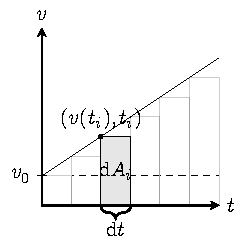
\includegraphics{integrals/simplemotionsubdivide}
        \caption{A subdivided graph}
        \label{fig:simplemotionsubdivided}
    \end{subfigure}
    \begin{subfigure}[b]{0.45\textwidth}
        \centering
        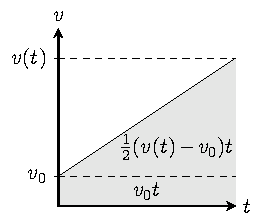
\includegraphics{integrals/simplemotionr}
        \caption{A graph showing the area of the gray trapezoid broken into two parts}
        \label{fig:simplemotionr}
    \end{subfigure}
    \caption{A $v$-$t$ graph of a ball dropped from a building}
\end{figure}

\begin{multicols}{2}
A good strategy in math if you don't know what to do is to just graph the function. The graph of \cref{eq:simplemotionr2} is shown in \cref{fig:simplemotionsubdivided}. A small time interval represents a little step in the $t$ axis. The curve shown in the graph represents $\vv{g}t + \vv{v}_0$. Therefore, $\odif{t}(\vv{g}t + \vv{v}_0)$ would just represent an area of a little rectangle $\odif{A}$ as shown in the figure.

The total change in position is the sum all those rectangles. When $\odif{t} \appr 0$, the sum of all $\odif{t}(\vv{g}t + \vv{v}_0)$ approaches the area under the graph, which can be calculated geometrically as shown in \cref{fig:simplemotionr}. Thus,
\begin{align}
    \vv{r} &= \frac{1}{2}(\vv{v}(t) - \vv{t}_0)t + \vv{v}_0t + C \\
    &= \frac{1}{2}(\vv{g}t - \vv{t}_0)t + \vv{v}_0t + C \\
    &= \frac{1}{2}\vv{g}\times t^2 + \vv{v}_0t + C
\end{align}
When $t = 0$, $\vv{r} = \vv{r}_0$. Therefore,
\begin{align*}
    \vv{r}_0 &= \frac{1}{2}\vv{g}\times 0^2 + \vv{v}_0\times 0 + C \\
    \vv{r}_0 &= C.
\end{align*}
Therefore,
\begin{equation}
    \vv{r}(t) = \frac{1}{2}\vv{g}t^2 + \vv{v}_0t + \vv{r}_0.
\end{equation}

To model the trajectory of the ball, we set
\begin{enumerate}[noitemsep]
    \item $\vv{v}_0 = 0$ (object is dropped and starts at zero speed)
    \item $\vv{r}_0 = 0$ (convenient initial condition placement)
\end{enumerate}
thus we get,
\begin{gather}
    \vv{r} = \frac{1}{2}\vv{g}t^2 \implies t = \sqrt{\frac{2\vv{r}}{\vv{g}}}
\end{gather}
\end{multicols}
Since the ground is at $\vv{r} = h$, the time that the ball hits the ground is then $\sqrt{2h/\vv{g}}$.

\subsection{Conclusion: area under the curve and antiderivative}

The form of the differential equation that we've solved is in the form $\odv{x}{t} = f(x)$. We have to undo the derivative, and the simplest way is to do separation of variables and turn the equation into
\begin{equation}
    \odif{x} = f(x)\odif{t},
\end{equation}
which reads,
\begin{quotation}
    A small change in $x$, i.e., $\odif{x}$ is represented by the area of a rectangle width $\odif{t}$ and height $f(x)$.
\end{quotation}
And, the total change $x$ is represented by the sum all those little rectangles, which is the area under the curve $f(x)$. Then, we add a constant $C$ to compensate for the initial condition. In symbolic form introduced in \cref{sec:brief_notation_of_calculus_integral}, it's just
\begin{align}
    \int\odif{x} &= \int g(x)\odif{t} \\
    x &= \int g(x)\odif{t}.
\end{align}

For now, we could say that integration is the reverse of derivatives. But to clearly see how this is linked for every function, we must study the fundamental theorem of calculus, which is the bridge between integration and differentiation.

Before we go there, let me clarify some terminologies. An \textbf{integral} refers to the area under the curve evaluated between two points. We say that an integral must have an \textbf{integral bound}. If we want to find the area under a function $f(x)$ from $x = a$ to $x = b$, we write it as
\begin{equation}
    A = \int_a^b f(x)\odif{x}.
\end{equation}
This just reads
\begin{quotation}
    The area $A$ under the curve $f(x)$ from $x = a$ to $x = b$ is equal to the sum of the area of many thin stripes width $\odif{x}$ height $f(x)$ that lies between $x = a$ and $x = b$.
\end{quotation}
The \textbf{antiderivative} however, refers to the function which takes in a value $a$, and output the integral of $f(x)$, evaluated from $0$ to $a$. Therefore, if $A(a)$ is the antiderivative of $f(x)$, then
\begin{equation}
    A(a) = \int_0^a f(x)\odif{x}.
\end{equation}
It also implies that if the area between $a$ and $b$ can be evaluated by
\begin{equation}
    \int_a^b f(x)\odif{x} = A(b) - A(a).
\end{equation}

\section{The fundamental theorem of calculus}
\label{sec:fundamentalthmofcalc}

\index{The fundamental theorem of calculus!first part}The intuition of fundamental theorem of calculus states that derivatives and integrals are essentially inverse of each other. In this section, I'll clarify this fact and make it more rigorous.
\begin{theorem}{The (first) fundamental theorem of calculus}{fundamentalthmofcalc1}
    If a function $f(x)$ has an antiderivative $A(x)$, then
    \begin{equation}
        \odv{A(x)}{x} = f(x).
    \end{equation}
\end{theorem}

\begin{figure}[b]
    \centering
    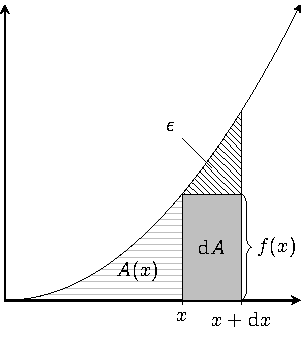
\includegraphics{integrals/fundamentalthmofcalc}
    \caption{The geometrical interpretation of part one of the fundamental theorem of calculus (\cref{theorem:fundamentalthmofcalc1}).}
    \label{fig:fundamentalthmofcalc}
\end{figure}
If $A(x)$ is the antiderivative of $f(x)$, then
\begin{equation}
    \int_{0}^{x} f(x)\odif{x} = A(x).
\end{equation}
The \emph{actual} area of one of the stripes (not rectangles) width $\odif{x}$ shown in \cref{fig:fundamentalthmofcalc}, it's obviously $A(x + \odif{x}) - A(x)$. The riemann sum approximation approximates the area by a small rectangle area $f(x)\odif{x}$. We can write the relation between the actual and the approximated area as
\begin{equation}
    A(x + \odif{x}) - A(x) \approx f(x)\odif{x}.
\end{equation}
To turn this into an equality, we add a correction term $\epsilon$
\begin{equation}
    A(x + \odif{x}) - A(x) = f(x)\odif{x} + \epsilon.
\end{equation}
If we let $\odif{x} \appr 0$, $\epsilon$ is negligible compared to $f(x)\odif{x}$; therefore,
\begin{equation}
    \lim_{\odif{x} \appr 0}A(x + \odif{x}) - A(x) = \lim_{\odif{x} \appr 0}f(x)\odif{x}.
\end{equation}
Since $f(x)$ is not a variable that's controlled by the limit sign,
\begin{align*}
    \lim_{\odif{x} \appr 0}A(x + \odif{x}) - A(x) &= f(x)\lim_{\odif{x} \appr 0}\odif{x} \\
    \lim_{\odif{x} \appr 0}\frac{A(x + \odif{x}) - A(x)}{\odif{x}} &= f(x).
\end{align*}
And here, we see that the L.H.S. is just the derivative of $A(x)$ w.r.t. $x$, thus
\begin{equation}
    \odv{A(x)}{x} = f(x),
\end{equation}
or ``\textit{the rate of change in area is the function itself}''. But the area function is given by the integral. This means
\begin{equation}
    \odv{x}\int f(x)\odif{x} = f(x):
\end{equation}
integrals and derivatives are inverses of each other. If we rephrase \cref{theorem:fundamentalthmofcalc1}, we see that ``\textit{the integral is the cumulative effect of the function}.''

\index{The fundamental theorem of calculus!second part}The second fundamental theorem of calculus,
\begin{theorem}{The second fundamental theorem of calculus (Newton-Leibniz rule)}{fundamentalthmofcalc2}
    If a function $f(x)$ has an antiderivative $A(x)$, then its indefinite integral from $a$ to $b$ is
    \begin{equation}
        \int_{a}^{b}f(x)\odif{x} = \int_{0}^{b}f(x)\odif{x} - \int_{0}^{a}f(x)\odif{x} = A(b) - A(a).
    \end{equation}
\end{theorem}
follows as a direct consequence of the geometrical interpretation of integrals: area under the curve.

The fundamental theorem of calculus allows us to evaluate integrals using derivatives. For example, if the derivative of $x^2$ is $2x$, then we also know that the integral of $2x\odif{x}$ is just $x^2$, which we'll discuss how to do that in the next chapter.

\section{How to calculate an integral? Riemann sum}
\label{sec:riemann_sum}

\begin{figure}[b]
    \centering
    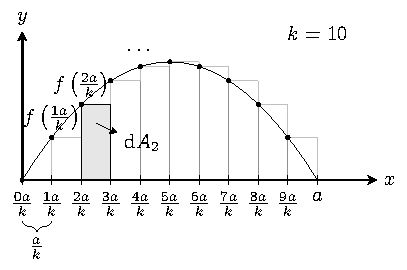
\includegraphics{integrals/integralex}
    \caption{Illustration of Riemann sum of a function $f(x)$ from $0$ to $a$ by setting $k = 10$}
    \label{fig:integralex1}
\end{figure}

In \cref{sec:function_in_the_haystack}, we used geometry to find the area under a curve. However, that is not always possible, e.g., try integrating \cref{fig:integralex1} geometrically\footnote{This is what you'd get if you solve the simple harmonic oscillator}. It'd be impossible. But we can still approximate its area by slicing the area under the curve into thin rectangular stripes, then summing them. The approximated area is called the \index{Riemann sum}\textbf{Riemann sum}. Due to its computational cost, you don't really want to use this method. However, to develop a good intuition at the integral, we should still know its symbolic form.

Let there be a function $A(s)$ that represents the actual area of a function $f(x)$ from $0$ to $s$. The approximated area is then
\begin{equation}
    \sum_{i = 0}^{k}\odif{A_i} = \sum_{i = 0}^{k}\mathrm{width} \times \mathrm{height}
\end{equation}
where $k$ is the amount of subdivisions. From \cref{fig:integralex1}, the width of each stripe is $\flatfrac{a}{k}$, and the height of the $i$'th stripe is $f(\flatfrac{ia}{k})$. Therefore,
\begin{equation*}
    \sum_{i = 0}^{k}\frac{a}{k}\times f\left(\frac{ia}{k}\right).
\end{equation*}

In \cref{fig:integralex1}, we  $k = 10$. The area of the second rectangle $\odif{A_2}$ is
\begin{equation*}
    \odif{A_2} = \frac{a}{k}f\left(\frac{2a}{k}\right).    
\end{equation*}

For an arbitrarily finite $k$, the Riemann sum is just an approximation. If you want to find the \textit{actual} area under the curve, let $k \appr \infty$. The limit as $k \appr \infty$ is what we actually call the \textbf{integral}. Thus, we say
\begin{df}{Naive definition of integrals}{integralsnaivedefinition}
    The \index{integrals!definite integrals}(definite) integral, or the area under the curve of $f(x) = y$ from $0$ to $a$, is defined as
    \begin{equation}
        \int_{0}^{a}\odif{A} = \int_{0}^{a}f(x)\odif{x} = \lim_{k \appr \infty}\sum_{i = 0}^{k}\frac{a}{k} \times f\left(\frac{ia}{k}\right) = A(a).
    \end{equation}
    where $\int$ is the integral sign\footnote{Famously known for looking like a beansprout}. Here, $0$ is the lower bound of integration, and $a$, the higher bound. The function $A(x)$ is called the \textbf{antiderivative}, or the \index{integrals!indefinite integrals}\textbf{indefinite integral} of $f(x)$.
\end{df}

I shall put these definitions into perspective in the next two examples. It might use a bit of series knowledge. If you don't know, you can simply search up the summation identities that I'll use in \emph{Wikipedia} \cite{wikipedia-summation}.

\begin{exmp}{Riemann sum and antiderivative of $x^2$}{}
    Let $f(x) = x^2$, and let $A(a)$ be the antiderivative of $f(x)$, i.e., $A(a)$ is the area under the curve of $f(x)$ from $0$ to $a$. Note that
    \begin{equation}
        \sum_{i = 0}^{k}i^2 = \frac{k(k + 1)(2k + 1)}{6},
    \end{equation}
    The Riemann sum is then
    \begin{align}
        \sum_{i = 0}^{k}\frac{a}{k}&\times f\left( i a \over k \right) = \sum_{i = 0}^k\frac{a}{k}\times \left(ia\over k\right)^2 \\
        &= \sum_{i = 0}^k\frac{a^3}{k^3}\times i^2 \\
        &= \frac{a^3}{k^3}\times \frac{k(k + 1)(2k + 1)}{6}.
    \end{align}
    To find the antiderivative, let $k \appr \infty$. Notice that the $+1$ in the parenthesis are negligible when $k \appr \infty$. Therefore, we can write the antiderivative as
    \begin{align}
        A(a) &= \int_0^a f(x)\odif{x} \\
        &= \lim_{k \appr \infty}\frac{a^3}{k^3}\times \frac{k(k + 1)(2k + 1)}{6} \\
        &= \lim_{k \appr \infty}\frac{a^3}{k^3}\times \frac{2k^3}{6} \\
        &= \lim_{k \appr \infty}\frac{x^3}{3} = \frac{x^3}{3}.
    \end{align}
\end{exmp}

\begin{exmp}{Riemann sum and antiderivative of $x^3$}{}
    Let $f(x) = 4x^3$, and let $A(a)$ be the antiderivative of $f(x)$, i.e., $A(a)$ is the area under the curve of $f(x)$ from $0$ to $a$. Note that
    \begin{equation}
        \sum_{i = 0}^{k}i^3 = \left(\frac{k(k + 1)}{2}\right)^2,
    \end{equation}
    The Riemann sum is then
    \begin{align*}
        \sum_{i = 0}^{k}\frac{a}{k}&\times f\left( i a \over k \right) = \sum_{i = 0}^k\frac{a}{k}\times 4\left(ia\over k\right)^3 \\
        &= 4\sum_{i = 0}^k \left(\frac{x}{k}\right)^4 i^3 \\
        &= 4\left(\frac{x}{k}\right)^4\left(k(k+1)\over 2\right)^2.
    \end{align*}
    To find the antiderivative, let $k \appr \infty$. The $+1$ in $(k + 1)$ can be ignored as $k \appr \infty$. Therefore,
    \begin{align*}
        A(a) &= \int_0^a f(x)\odif{x} \\
        &= \lim_{k\appr\infty}4\left(x\over k\right)^4\left(k^2\over 2\right)^2 \\
        &= \lim_{k\appr\infty}x^4 = x^4.
    \end{align*}
\end{exmp}

\section{Basic applications of the integrals}

\subsection{Five equations of linear motion}
\label{sec:fiveequationsoflinearmotion}

\index{equation of motion!uniformed acceleration}So far, we have developed an intuition for derivatives, integrals, and their relationship. Let's apply those concepts to derive the famous equations of linear motion:
\begin{gather}
    v(t) = v_0 + at, \label{eq:linearmotion1}\\
    s = \frac{1}{2}(v_0 + v(t))t, \label{eq:linearmotion2}\\
    s = v_0(t)t + \frac{1}{2}at^2, \label{eq:linearmotion3}\\
    s = v(t)t - \frac{1}{2}at^2,\label{eq:linearmotion4}\\
    v(t)^2 = v_0^2 + 2as. \label{eq:linearmotion5}
\end{gather}

\begin{figure}[b]
    \centering
    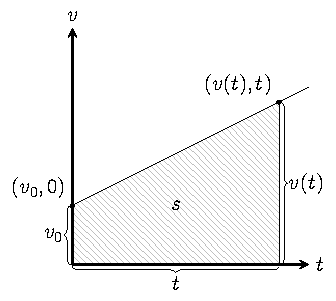
\includegraphics{integrals/constantacceleration}
    \caption{$v$-$t$ graph of an object under constant or uniformed acceleration}
    \label{fig:vtconstantacceleration}
\end{figure}
Here, $v_0$ represents the initial velocity, $v(t)$, the velocity at any time $t$, $a$, the acceleration, and $s$, the displacement. These equations are derived from the Newton's second law on \emph{constant/uniformed acceleration} motion in one dimension, which we can evaluate using the geometrical interpretation of integrals developed earlier.

Because we've constrained the object to accelerate at $a$, the force exerted must be $ma$. Newton's second law $F = m\odv[ord = 2]{x}{t}$ then simplifies to $a = \odv[ord = 2]{x}{t}$. The same idea applies, we rewrite the equation in terms of $v$.
\begin{equation}
    a = \odv{v}{t} \label{eq:linearmotionintermediate}
\end{equation}
Which reads, ``\emph{the rate of change of $v$ w.r.t. $t$ is $a$}'' or ``\emph{the slope of the $v$-$t$ curve is always equals to $a$}''. Because $a$ is constant, the $v$-$t$ curve must be a straight line with slope $a$, shown in \cref{fig:vtconstantacceleration}.

\begin{multicols}{2}
\begin{proof}[Derivation of \cref{eq:linearmotion1}]
    We take advantage of the linearness of the curve. Just pick two points on \cref{fig:vtconstantacceleration}, as already shown, then
    \begin{align*}
        m = a &= \frac{\Delta v}{\Delta t} = \frac{v(t) - v_0}{t - 0} \\
        a & = \frac{v(t) - v_0}{t} \\
        v(t) &= v_0 + at.\qedhere
    \end{align*}
\end{proof}

\begin{proof}[Derivation of \cref{eq:linearmotion2}] 
    Use the reverse of \cref{theorem:fundamentalthmofcalc1}. We know that\footnote{Here, $x$ is replaced with $s$ to represent displacement in one dimension.} $v = \odv*{s}{t}$; therefore,
    \begin{equation*}
        \int v\odif{t} = s,
    \end{equation*}
    which reads ``\emph{The displacement $s$ is the area under the curve of a $v$-$t$ graph}''. From \cref{fig:vtconstantacceleration}, the area under the curve is a trapezoid with side length $v_0$, $v(t)$, and width $t$. Thus,
    \begin{equation*}
        s = \frac{1}{2}(v_0 + v(t))t,
    \end{equation*}
    which is just \cref{eq:linearmotion2}: the area of a trapezoid.
\end{proof}

\begin{proof}[Derivation of \cref{eq:linearmotion3,eq:linearmotion4,eq:linearmotion5}]
    We can arrange \cref{eq:linearmotion1} into three different ways, then plug in \cref{eq:linearmotion2}.
    First, $v(t) = v_0 + at$
    \begin{align*}
        s &= \frac{1}{2}(v_0 + v_0 + at)t \\
        &= v_0t + \frac{1}{2}at^2. 
    \end{align*}
    Second, $v_0 = v(t) - at$
    \begin{align*}
        s &= \frac{1}{2}(v(t) - at + v(t))t \\
        &= v(t)t - \frac{1}{2}at^2. 
    \end{align*}
    Third, $\displaystyle{t = \frac{v(t) - v_0}{a}}$
    \begin{align*}
        s &= \frac{1}{2}(v(t) + v_0)\frac{(v(t) - v_0)}{a} \\
        2as &= (v(t) + v_0)(v(t) - v_0) \\
        2as &= v(t)^2 - v_0^2 \\
        v(t)^2 &= 2as + v_0^2. \qedhere
    \end{align*}
\end{proof}
\end{multicols}

\subsection{The area of a circle}
\begin{figure}[t]
    \centering
    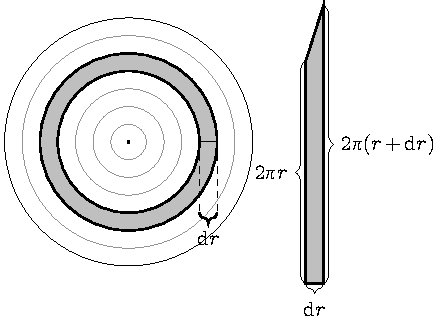
\includegraphics{integrals/dissectingcircle}
    \caption{(Left) Dissecting a circle radius $R$ radially into rings, each ring $\odif{r}$ thin. (Right) Stretching a ring into a trapezoid (Not to scale).}
    \label{fig:dissectingcircle}
\end{figure}

The perimeter of the circle is $2\cpi r$. For now, we only know how to find areas of polygons, but we want to know the circle's area. So, is there any way to turn a circle into a polygon? From \cref{sec:riemann_sum}, that the riemann sum can approximate areas under the curve using rectangular stripes. It'd be great if this circle can be turned into multiple rectangular stripes on a graph right?

So, we dissect a circle radially into small rings $\odif{r}$ thin, as shown in \cref{fig:dissectingcircle}. Then, stretch all the rings into a very thin trapezoid-like shape. It might seem impossible at first, but considering that our ring is very thin, it's quite easy to stretch it without breaking. I encourage you to grab a piece of paper, cut a really thin ring and try it out. If you actually do it, it'll look a bit warped. However, the warpedness will go away the thinner you go.

Since we sliced our trapezoid from a circle, for a stripe positioned at $r$, the inner side will be $2\cpi r$ long and the outer side, $2\cpi (r + dr)$. The area of the little trapezoid $\odif{A}$ then becomes
\begin{align*}
    \odif{A} &= \frac{1}{2}\odif{r}(2\cpi r + 2\cpi (r + dr)) \\
    &= 2\cpi r\odif{r} + 2\cpi\odif{r}^2. 
\end{align*}
As $\odif{r} \appr 0$, $\odif{r}^2$ becomes negligible. Therefore,
\begin{equation}
    \odif{A} = 2\cpi r \odif{r}.
\end{equation}
\begin{wrapfigure}[17]{r}{0.4\textwidth}
    \centering
    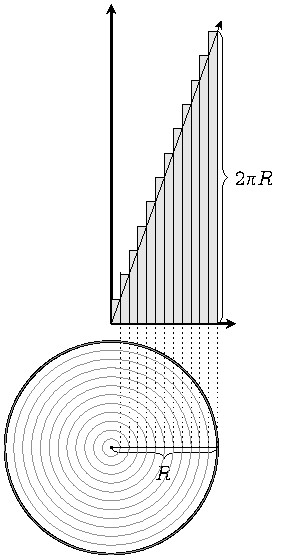
\includegraphics{integrals/dissectingcircle2}
    \caption{Rearranging all the approximated rectangles onto a graph (Not to scale).}
    \label{fig:dissectingcircle2}
\end{wrapfigure}
This equation says that for $\odif{r} \appr 0$, the trapezoid becomes a rectangle side length $\odif{r}$ and $2\cpi r$. Now, we have to sum it together. If we can put all these rectangles onto a graph, we can easily use the Riemann's sum to evaluate it. A natural way to do this is to put all the rectangles that we got from stretching the rings of the circle onto a graph one by one. The result would look something like \cref{fig:dissectingcircle2}\footnote{Not to scale}.

For every stripe at $r$, its height is $2\pi r$. If you were to plot the height of all rectangles when $\odif{r} \appr 0$, it'll eventually look like a curve that's given by $f(r) = 2\pi r$. We're interested in the area of the circle from $0$ to $R$. Now, it's transformed into the area under the curve of $f(r) = 2\pi r$: a triangle with base $R$ and height $f(R) = 2\pi R$. Thus, the area of a circle becomes
\begin{equation*}
    A = \frac{1}{2}R(2\pi R) = \pi R^2.
\end{equation*}

And there you go, you've turned essentially turned circle into a triangle and evaluate its area from there. I'd like to end off this chapter by mentioning the spirit of mathematics. Sometimes, you can't solve the problem directly. Most of the time, you have to re-frame the problem into another more-solvable problem. Problems like these often have the most sublime connections to the foundations of mathematics. This is a common theme in most of mathematics, especailly calculus. So, be sure to keep this in mind while reading through.

\conclusion

\begin{enumerate}
    \item Riemann sum are used to approximate areas under the curve of a function by using little rectangles then summing it.
    \item Integrals or anti-derivatives are functions that output the area under the graph of other functions.
    \item The limit where the width of the rectangles in the Riemann sum approaches zero, the Riemann sum becomes an integral.
    \item Integrals are the cumulative effect of a function.
    \item Integrals and derivatives are inverses of each other, and they're related by the fundamental theorem of calculus
    \item Integrals can be used in various ways by reframing questions into another simpler question.
\end{enumerate}